\section{径迹判选和电子鉴别}
在每次54.4 GeV 金-金对撞当中,末态平均有几百条径迹被STAR探测器所探测到。为了从中挑选出合格的电子径迹用来进行最后的分析,一些关于径迹质量和粒子鉴别的判选条件被应用在了本分析当中。下面的章节将对这两组判选条件进行详细的介绍。
\subsection{径迹判选}
\label{chap:track_selection}
在本分析中,主要用到的子探测器是时间投影室和飞行时间探测器。由于探测器本身的限制,分析中所用到的径迹应该在这两个探测器的接收度范围内,且可以被探测器很好地重建出来。
这样一来,分析中所用到的进行电子对重建的电子的径迹应该满足探测器接收度和径迹重建质量上的需求,从而保证整个分析的质量。

对于一条满足径迹重建质量要求的径迹来说,其对应的粒子在穿越时间投影室的过程中应该留下了足够多的击中来进行径迹重建。自然在本分析当中就对径迹用来重建的击中数(nHitsFit)有了要求。当两条粒子的径迹在空间位置上很近的时候,这两个粒子在时间投影室中留下的击中就容易被算法认为属于同一个粒子留下的径迹中的击中。为了避免这种情况,一条径迹用来重建的击中数和最大可利用击中数的比值(nHitsfit/nHitsPoss)应该大于0.52。时间投影室是利用粒子穿过漂移区域时的电离能损信息来进行粒子鉴别的,其具体方法在\ref{chap:TPC}当中已进行过讨论。那么和重建类似,一条满足径迹重建质量要求的径迹也需要留下足够多的击中来进行能量损失的计算,这也就对径迹用来计算电离能损的击中数(nHitsDedx)有了要求。
在本分析当中所研究的电子对都来源于夸克胶子等离子体或者短寿命的介子衰变,这意味着电子应该来源于主碰撞顶点(Primary Vertex)而不是离主碰撞顶点较远的次级衰变顶点。为了满足这个要求,一个关于径迹到主碰撞顶点的最近距离(distance of closest approach,DCA)的盘旋条件被添加到了分析当中。

详细的径迹质量判选条件和径迹的接收度范围在表\ref{tab:TrackQuality}左栏中列出。

\begin{table}[h!]
    \centering
    \caption{径迹质量和电子鉴别(eID)判选条件}
    \label{tab:TrackQuality}
    \begin{tabularx}{0.8\textwidth} {
    | >{\centering\arraybackslash}X |>{\centering\arraybackslash}X | }
        \hline
        径迹质量判选 & 电子鉴别(eID)   \\
        \hline
        $0.2 \leq p_{T} \leq 30 GeV/c $ & $p<0.8 GeV/c $ \\
        $|\eta| \leq 1 $ & $ 3*p - 3.15 \leq |n\sigma_{e}| \geq 2.0$  \\
        $dca \leq 1cm $ & $p \geq 0.8 GeV/c $\\ 
        $N_{HitsFit} \geq 20 $  & $ -0.75 \leq |n\sigma_{e}| \geq 2.0 $\\
        ${N_{HitsFit}}/{N_{HitsPoss}} \geq 0.52 $ &  $|1-1/\beta| < 0.25 $\\
        $N_{HitsDedx} \geq 15 $  & \\
        \hline
    \end{tabularx}
\end{table}

\subsection{电子鉴别(eID)}
\label{ch:eID}
当选出了符合径迹重建质量要求的径迹之后,再通过径迹的电离能损和速度信息就可以辨别出来径迹有没有可能为一条由电子留下来的径迹。
将每条径迹由时间投影室测量得到的电离能损和通过Bethe-Bloch公式计算得到的电子电离能损相比较后再由探测器的分辨率进行归一化便可以得到一个用来表明径迹为电子径迹的可能性的一个值,\nSigmaE 。具体计算公式如式\ref{eq:nSigmaE}所示。在理想情况下,电子的$n\sigma_\mathrm{e}$应该为一个中心值为0宽度为1的高斯分布。在径迹的动量比较高的时候,电子在工作气体中的电离能损和其他粒子重合,无法单独通过电离能损鉴别粒子。这时可以通过结合电离能损和飞行时间探测器所测得的速度信息来进行粒子鉴别。因为电子质量轻于其它强子,在相同动量下电子的速度会大于其他强子。这就意味着可以额外添加一个$1/\beta$的判选条件来进行电子鉴别。电子鉴别的条件在表\ref{tab:TrackQuality}的右栏列出。图 \ref{beta_Cut}和\ref{fig:nSigmaEwTOF}分别为$1/\beta$的分布和加上$1/\beta$判选条件后的$n\sigma_\mathrm{e}$分布。

\begin{equation}
    \label{eq:nSigmaE}
    n\sigma_e = \frac{log(\frac{dE/dx_{measure}}{dE/dx_{BB}})}{\sigma_{dE/dx}}
\end{equation}

\begin{figure}[htb]
    \centering
    \begin{subfigure}[b]{0.45\textwidth}
        \centering
        \includegraphics[width=\textwidth,clip]{figures/Chapter4/nSigmaEwTOF.png}
        \caption{}
        \label{fig:nSigmaEwTOF}
    \end{subfigure}
    \hfill
    \begin{subfigure}[b]{0.49\textwidth}
        \centering
        \includegraphics[width=\textwidth,clip]{figures/Chapter4/beta_Cut.png}
        \caption{}
        \label{fig:beta_Cut}
    \end{subfigure}
       \caption[\nSigmaE 和 $1/\beta$判选条件示意图]{图\ref{fig:nSigmaEwTOF}为\nSigmaE 判选条件示意图,其中黑色虚线为\sNN = 54.4GeV 中 \nSigmaE 的判选条件上下限。图 \ref{fig:beta_Cut}为$1/\beta$判选条件示意图, 黑色实线为判选条件上下限 }
       \label{fig:eID_cut}
\end{figure}

\subsection{电子样本纯度}
\label{chap:pruity}

从图\ref{fig:nSigmaEwTOF}可以看到,尽管通过\nSigmaE 和$1/\beta$的判选条件可以有效的选出电子样本,但仍然有一部分强子的\nSigmaE 分布会和电子的有所覆盖。这样就需要估计强子在电子样本当中所占的比重,即强子污染(hadron contamination)。

为了估计强子污染,首先要得到纯的强子以及电子样本的\nSigmaE 分布。这就需要通过某种方法挑选出纯强子和纯电子的数据样本,在本分析中纯强子样本是通过添加一个严苛的质量判选条件和比较宽松的$n\sigma_{hadron}$判选条件的方法挑选得到的。对于不同的强子,其质量判选条件在表\ref{tab:pure_sample}当中列出。当两条径迹的电荷相同、动量相似的时候,这两条径迹在时间投影室当中留下的击中会非常接近,这就使得这两条径迹在重建的时候很容易被重建成一条径迹,这就是merged track。在金-金对撞当中,因为末态大多数的带电粒子为$\pi$介子,所以我们在选取纯强子样本的时候把merged $\pi$也一并考虑了进来。
图\ref{fig:pure_hadron_sample}中为纯$\rm{\pi/k/p}$样本以及 merged $\pi$ 样本的$\rm{n\sigma_{e}~v.s.~p}$的二维分布。

\begin{table}[]
    \centering
    \caption{选取纯$\rm{\pi/k/p}$样本时的质量判选条件}
    \begin{tabular}{|c|c|}
        \hline
        particle & mass cut  \\
        \hline
        $\pi$ & $ 0.019 \pm 0.003 GeV/c^2$\\
        \hline
        $Kaon$ & $ 0.243 \pm 0.005 GeV/c^2$\\
        \hline
        $Proton$ & $ 0.879 \pm 0.020 GeV/c^2$ \\
        \hline
    \end{tabular}
    \label{tab:pure_sample}
\end{table}

\begin{figure}[h!]
    \centering
    \begin{subfigure}[h!]{0.43\textwidth}
            \includegraphics[width=\textwidth]{figures/Chapter4/PurePion.png}
            \caption{}
            \label{fig:PurePion}
    \end{subfigure}
    \begin{subfigure}[h!]{0.43\textwidth}
            \includegraphics[width=\textwidth]{figures/Chapter4/PureKaon.png}
            \caption{}
            \label{fig:PureKaon}
    \end{subfigure}

    \begin{subfigure}[h!]{0.43\textwidth}
            \includegraphics[width=\textwidth]{figures/Chapter4/PureProton.png}
            \caption{}
            \label{fig:PureProton}
    \end{subfigure}
    \begin{subfigure}[h!]{0.43\textwidth}
            \includegraphics[width=\textwidth]{figures/Chapter4/PureMergePion.png}
            \caption{}
            \label{fig:PureMergePion}
    \end{subfigure}
    \caption[纯$\rm{\pi/k/p}$样本以及 merged $\pi$ 样本的$\rm{n\sigma_{e}~v.s.~p}$的二维分布]{纯$\rm{\pi/k/p}$样本以及 merged $\pi$ 的  $\rm{n\sigma_{e}~v.s.~p}$的二维分布。左上:$\pi$介子;右上:K介子;左下:质子;右下:merged $\pi$ }
    \label{fig:pure_hadron_sample}
\end{figure}

而纯电子样本是通过挑选来自于$\pi^0$的Dalitz衰变以及光子转换的电子对得到的。如\ref{chap:photon_conversion}小节当中所讨论的一样,光子击中探测器材料所产生的正负电子对其质量应该为0,但因为primary track要求通过碰撞顶点的原因导致其重建出来之后有一个很小的不变质量。这样如果选取不变质量很小的双电子对来选取纯电子数据样本。
在本分析中所用到的挑选纯电子数据样本的判选条件为$\rm{M_{ee} < 0.015~GeV/c^2}$,如图\ref{fig:PureElectron_cut}所示。在图中可以看到在这个质量区间内双电子信号的信噪比很高,在0-80\%中心度下可以达到129.97的信噪比,纯电子数据样本的$n\sigma_e$分布如图\ref{fig:PureElectron_Sample}所示。

\begin{figure}[h!]
    \centering
    \begin{subfigure}[h!]{0.45\textwidth}
            \includegraphics[width=\textwidth]{figures/Chapter4/PureElectron_cut.png}
            \caption{}
            \label{fig:PureElectron_cut}
    \end{subfigure}
    \begin{subfigure}[h!]{0.45\textwidth}
            \includegraphics[width=\textwidth]{figures/Chapter4/PureElectron_Sample.png}
            \caption{}
            \label{fig:PureElectron_Sample}
    \end{subfigure}
    \caption[纯电子数据样本选取的判选条件以及纯电子样本的$\rm{n\sigma_{e}~v.s.~p}$的二维分布]{纯电子数据样本选取的判选条件(左图)以及纯电子样本的$\rm{n\sigma_{e}~v.s.~p}$的二维分布(右图)}
    \label{fig:PureElectron_sample_total}
\end{figure}

在得到纯强子以及纯电子数据样本之后,就可以在不同的动量区间内通过拟合的方式得到各个粒子样本在不同区间内$n\sigma_{e}$分布的中心值和宽度。结果如图\ref{fig:MeanAndSigma_puresample}所示。基于这些结果,可以通过对总的数据样本进行多高斯拟合的方式来确定不同动量区间内的电子纯度。

\begin{figure}[h!]
    \centering
    \begin{subfigure}[h!]{0.45\textwidth}
            \includegraphics[width=\textwidth]{figures/Chapter4/Mean_pureSample.png}
            \caption{}
            \label{fig:Mean_pureSample}
    \end{subfigure}
    \begin{subfigure}[h!]{0.45\textwidth}
            \includegraphics[width=\textwidth]{figures/Chapter4/Sigma_PureSample.png}
            \caption{}
            \label{fig:Sigma_PureSample}
    \end{subfigure}
    \caption[不同粒子样本在不同动量区间内的$n\sigma_{e}$分布中心值以及宽度示意图]{不同粒子样本在不同动量区间内的$n\sigma_{e}$分布中心值(左图)以及宽度(右图)示意图}
    \label{fig:MeanAndSigma_puresample}
\end{figure}

从\label{fig:Mean_pureSample}可以看出,强子样本的$n\sigma_{e}$分布的中心值和电子样本的$n\sigma_{e}$分布中心值仍然有重叠的区间,这就导致
在进行多高斯拟合时,其单个高斯分布的产额在中心值重叠的区间会变得不稳定。以图\ref{fig:MultGaus_CorssOver_Region}中的分布为例,在这个动量区间内质子和电子的分布中心值以及宽度基本重合,这就导致二者的产额在实际拟合过程中可以被相对随机地分配。为了避免这样的问题发生,对总体数据进行了两轮的多高斯拟合,通过第一轮拟合来估计强子在不同区间内的产额,从而保证粒子的产额在拟合过程中保持稳定。
\begin{figure}[h!]
    \centering
    \begin{subfigure}[h!]{0.45\textwidth}
            \includegraphics[width=\textwidth]{figures/Chapter4/MultGaus_good.png}
            \caption{}
            \label{fig:MultGaus_good}
    \end{subfigure}
    \begin{subfigure}[h!]{0.45\textwidth}
            \includegraphics[width=\textwidth]{figures/Chapter4/MultGaus_CorssOver_Region.png}
            \caption{}
            \label{fig:MultGaus_CorssOver_Region}
    \end{subfigure}
    \caption[计算电子纯度的多高斯拟合在不同动量区间内拟合结果示意图]{计算电子纯度的多高斯拟合在不同动量区间内拟合结果示意图 左图质量区间: $ 0.72~<~p~<~0.76~GeV$.右图质量区间: $ 0.96~<~p~<~1.00~GeV$,其中右图的质量区间位于强子样本的$n\sigma_{e}$分布的中心值和电子样本的$n\sigma_{e}$分布有重叠的区间内}
    \label{fig:Multi-Gaussian}
\end{figure}

首先进行第一轮多高斯拟合,在这一轮拟合当中不同粒子的$n\sigma_{e}$高斯分布的中心值和宽度被固定为图\ref{fig:MeanAndSigma_puresample}中所示的值,仅有产额作为自由参数参与拟合。第一轮多高斯拟合结束之后可以得到各个粒子的产额随着动量变化的分布。如图\ref{fig:Fit_Interpolate_ConstValue_FirstRound}所示。可以看到,在$n\sigma_{e}$中心值有重叠的动量区间,产额拟合结果变得很不稳定。为了改进拟合的结果,在这些$n\sigma_{e}$分布有重叠的动量区间内对强子的产额进行指数拟合。在第二轮拟合当中,这些通过指数拟合得到的强子产额被设置为多高斯拟合时每个强子分量的产额参数并且固定,此时只有电子的产额会作为自由参数进行拟合,拟合结果如图\ref{fig:Fit_Interpolate_ConstValue}所示。
\begin{figure}[h!]
    \centering
    \begin{subfigure}[h!]{0.43\textwidth}
            \includegraphics[width=\textwidth]{figures/Chapter4/Fit_Interpolate_ConstValue_FirstRound.pdf}
            \caption{}
            \label{fig:Fit_Interpolate_ConstValue_FirstRound}
    \end{subfigure}
    \begin{subfigure}[h!]{0.43\textwidth}
            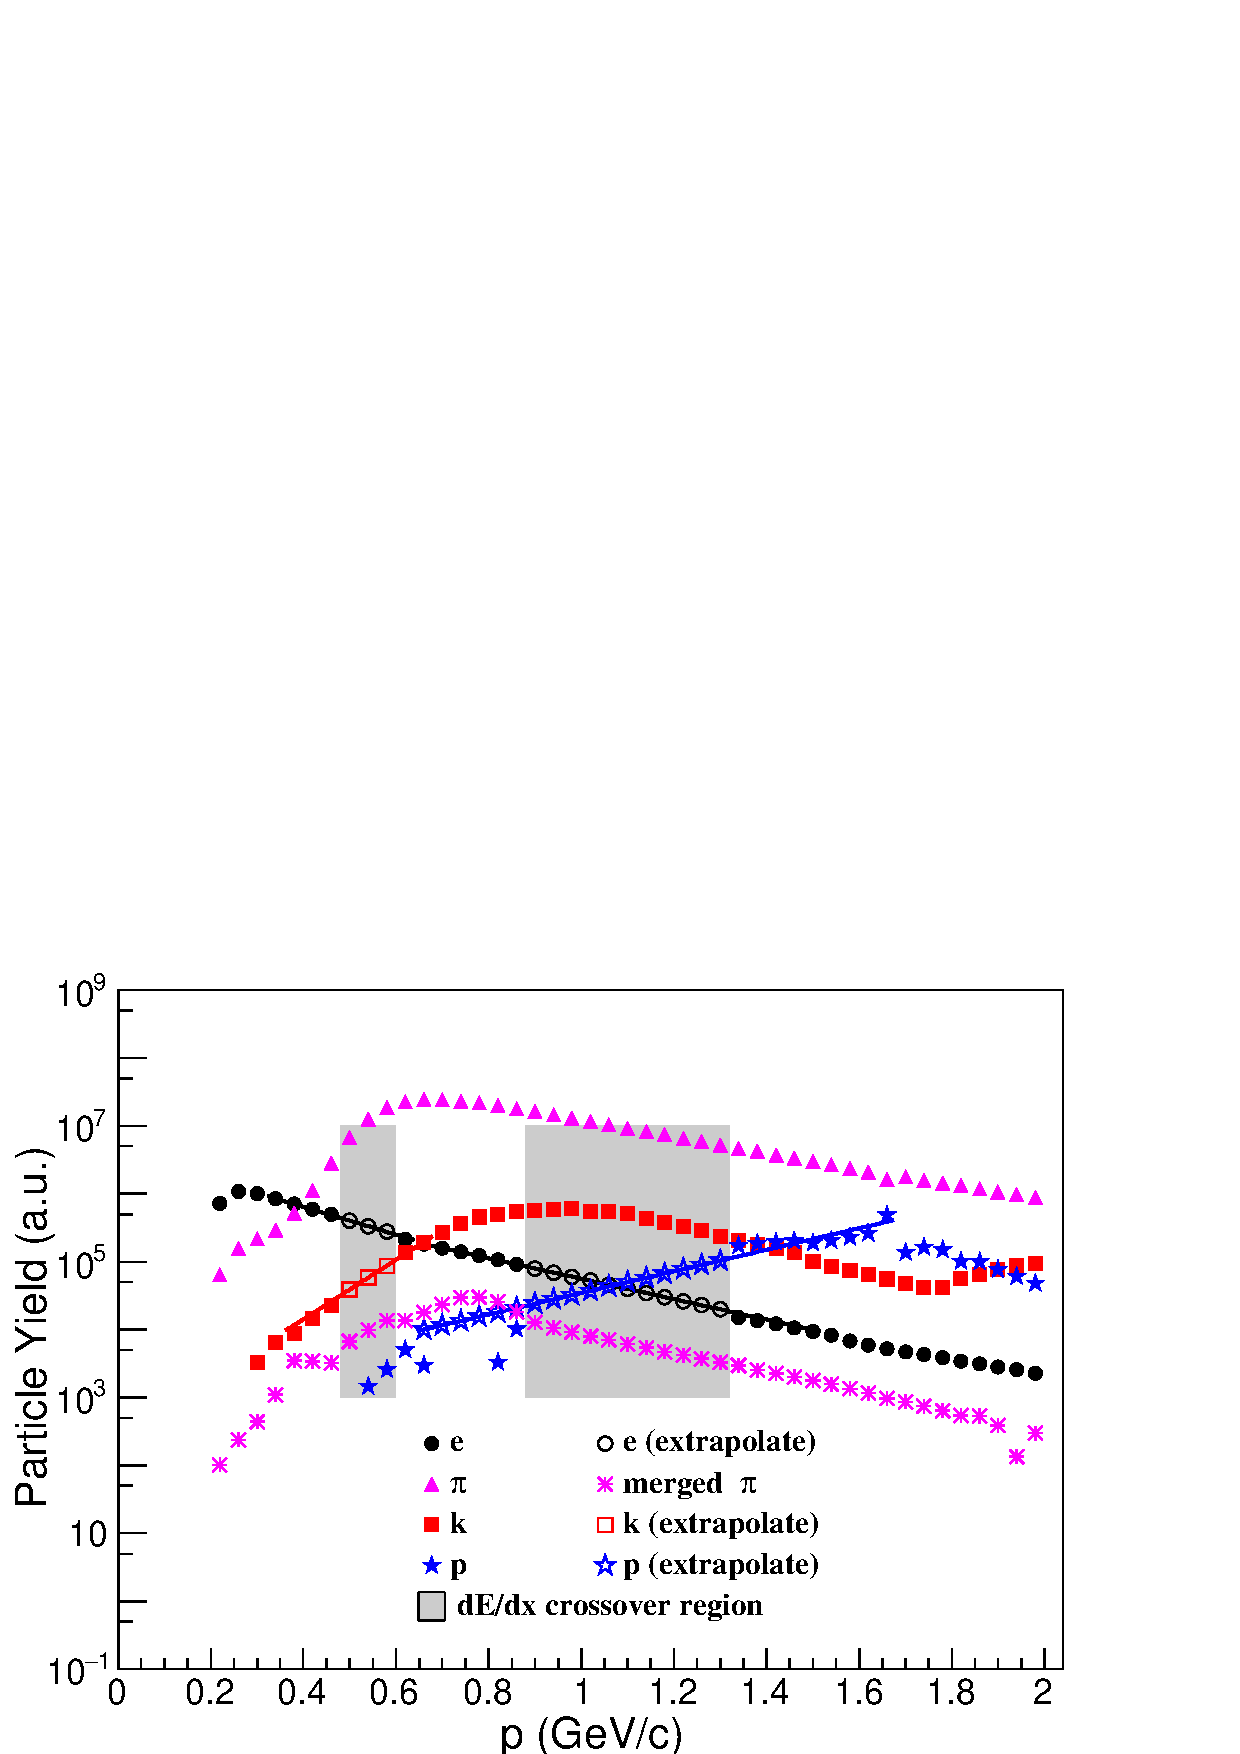
\includegraphics[width=\textwidth]{figures/Chapter4/Fit_Interpolate_ConstValue.pdf}
            \caption{}
            \label{fig:Fit_Interpolate_ConstValue}
    \end{subfigure}
    \caption[计算电子纯度时两轮高斯拟合的结果示意图]{计算电子纯度时两轮高斯拟合的结果示意图。左图为第一轮高斯拟合的结果,右图为第二轮高斯拟合的结果。灰色条带标出的区域为强子样本的$n\sigma_{e}$分布的中心值和电子样本的$n\sigma_{e}$分布有重叠的区间}
    \label{fig:Multi-Gaussian_result}
\end{figure}

在进行第二轮拟合的同时我们可以计算得到电子在各个动量区间内的纯度。为了验证拟合结果的准确性,电子的产额被单独画出,以检查第二轮拟合的结果是否符合预期要求,结果如图\ref{fig:Econst_crosscheck}所示。可以看到在第二轮拟合当中电子的产额分布是一个平滑的分布,符合预期要求。电子的纯度计算结果如图\ref{fig:nSigEcut4TpcE_Pur}所示,其中绿色的条带是第一轮拟合和第二轮拟合当中电子纯度的差值,被用作电子纯度的误差。灰色条带覆盖的区域即为强子样本的$n\sigma_{e}$分布的中心值和电子样本的$n\sigma_{e}$分布有重叠的区间。
\begin{figure}[h!]
    \centering
    \begin{subfigure}[h!]{0.43\textwidth}
            \includegraphics[width=\textwidth]{figures/Chapter4/Econst_crosscheck.pdf}
            \caption{}
            \label{fig:Econst_crosscheck}
    \end{subfigure}
    \begin{subfigure}[h!]{0.43\textwidth}
            \includegraphics[width=\textwidth]{figures/Chapter4/nSigEcut4TpcE_Pur.pdf}
            % \includegraphics{figures/Chapter4/nSigEcut4TpcE_Pur.pdf}
            \caption{}
            \label{fig:nSigEcut4TpcE_Pur}
    \end{subfigure}
    \caption[电子产额以及电子纯度示意图]{电子产额以及电子纯度示意图。左图为用以检查拟合结果稳定性的电子产额抽取结果;右图为电子纯度计算结果,绿色误差带为电子纯度计算时的系统,灰色条带标出了强子样本的$n\sigma_{e}$分布的中心值和电子样本的$n\sigma_{e}$分布有重叠的区间}
    \label{fig:Purity_check}
\end{figure}